\section{Introduction}
Inertial road-surface screening uses validation to choose a classifier and communicate its expected performance. An agency also needs to know how many road events the selected system detects and how many alarms it generates. These three outcomes can respond differently to a change in validation design: a higher-scoring selected classifier can have a less accurate performance estimate, and additional correct windows can occur within events that were already detected.

Low-cost pavement-sensing studies have examined measurement consistency across survey conditions \citep{sandamal2022,yu2023}. Road-event work has also studied generalisation to unknown vehicles, drivers and environments, including the original PVS investigation \citep{pvspaper}. Spatial, temporal and hierarchical validation distinguish acquisition relations that random withholding can retain \citep{roberts,ploton}. The practical question is how these validation choices affect candidate selection, the accuracy of its reported score and the resulting screening workload together.

We address this question with fixed-candidate experiments whose validation estimates are paired with the outer predictions of the same selected candidate. Nine PVS acquisitions provide controlled vehicle/driver and scenario holdouts. A separately collected Karlsruhe dataset supplies a final GPS-date group excluded from development, with spatial purging of repeated locations and matched inner training budgets \citep{pvsdata,kitpaper,kitdata}. The saved outer predictions then support annotation-interval detection and alarm counts. RoadSens source and temporal-representation experiments provide supporting evidence on evaluation scale and useful inertial information \citep{roadsens,roadsensdata}.

The core contribution is a controlled empirical account of three evaluation outcomes in pavement screening. First, nested comparisons distinguish selecting a stronger classifier from estimating its performance accurately, including disjoint-window and training-budget checks. Second, the independent-source date test examines the comparison under frozen choices and geographic separation. Third, event-level readouts establish when classification gains increase interval coverage or change notification burden. Figure~\ref{fig:graphical-abstract} presents the source-audit and nested-selection workflow; the Karlsruhe and event results extend its readouts.

\begin{figure}[!htbp]
\centering
\begin{singlespace}
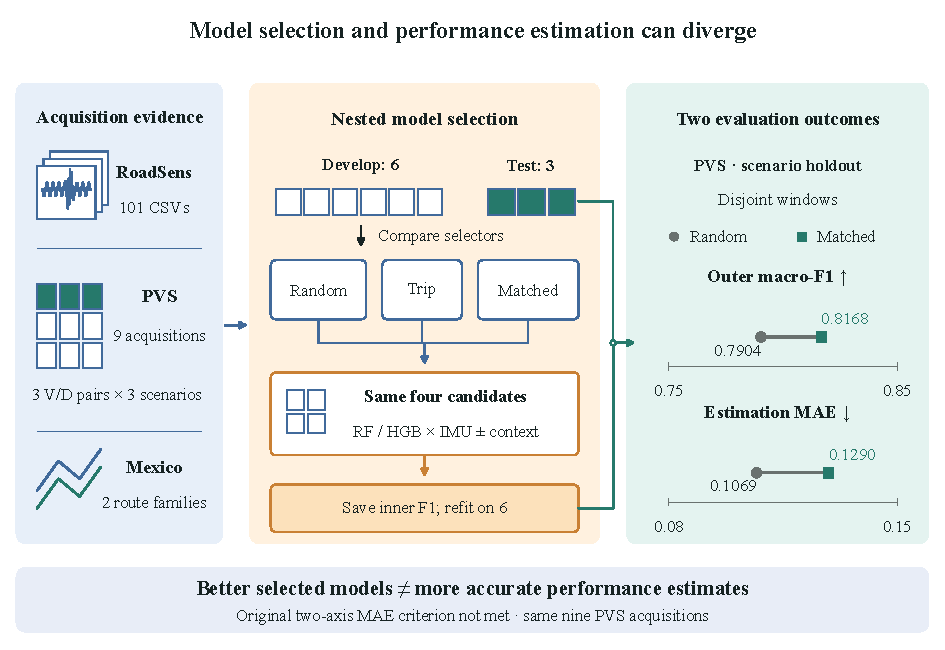
\includegraphics[width=\linewidth]{figures/graphical_abstract_v17.pdf}
\caption{Source audit and nested-selection workflow. RoadSens, PVS and Mexico/Puebla are separate source tasks; the Karlsruhe date test extends the evaluation. PVS develops on six acquisitions and tests on three. The right panel shows three-domain scenario means with disjoint windows: matched selection increases outer F1 and estimation MAE. Highlights, waveforms and route lines are schematic; V/D denotes vehicle/driver.}
\label{fig:graphical-abstract}
\end{singlespace}
\end{figure}

\section{Materials and methods}
\subsection{Paired selection and estimation endpoints}
For each validation scheme, candidates share exact eligible splits and fitted-row budgets. The candidate with the highest pooled inner out-of-fold (OOF) macro-F1 is selected, with a fixed candidate-order tie break. Its identity and inner estimate are saved before outer prediction. The candidate is refitted using development observations and assessed on the complete held-out domain.

Let $\widehat F_{s,d}$ be the saved estimate for selector $s$ in outer domain $d$, and $F^{\mathrm{out}}_{s,d}$ the outer macro-F1 of that same chosen candidate. We report selected-model classification performance and estimation error separately:
\begin{equation}
 \overline F^{\mathrm{out}}_s=\frac{1}{D}\sum_{d=1}^{D}F^{\mathrm{out}}_{s,d},
 \qquad
 E_s=\frac{1}{D}\sum_{d=1}^{D}\left|\widehat F_{s,d}-F^{\mathrm{out}}_{s,d}\right|.
\end{equation}
PVS has $D=3$ domains per axis. Karlsruhe has one final domain, so its error is one absolute discrepancy. Macro-F1 averages class-specific F1 with zero assigned to an undefined class term. Pooled OOF scores are calculated from combined held-out predictions; outer PVS summaries average the three domain scores. All datasets retain their own tasks and fitted models.

\subsection{PVS controlled acquisition holdouts}
PVS crosses three vehicle/driver pairs with three scenarios, yielding nine acquisitions \citep{pvsdata,pvspaper}. The binary target distinguishes released asphalt/cobblestone speed-bump intervals from \path{no_speed_bump}. Vehicle and driver are linked in the source design. We use six left-dashboard accelerometer/gyroscope axes at nominally 100 Hz. Trailing 100-row windows, evaluated every 25 rows, provide 30 axis-wise statistics: mean, population standard deviation, RMS, range and maximum absolute magnitude. A contextual variant adds anchor latitude, longitude and speed. The target is the final-anchor label, retaining exactly one active indicator. The primary population has 43,204 windows, including 682 positive anchors; a disjoint-window check has 10,804 windows from the same acquisitions.

The four candidates are random forest (RF100) and histogram gradient boosting (HGB), each with inertial-only or inertial-plus-context inputs. Settings are fixed across selectors: RF100 uses 100 trees, depth 20, minimum leaf size five and balanced class weights; HGB uses 100 iterations, up to 31 leaves, learning rate 0.1, L2 regularisation one, balanced classes and no early stopping. Median imputation is fitted only on actual training rows. A deterministic class-proportional cap limits fits to 20,000 windows. Full settings and feature order are in Supplementary Sections S11 and S15.

An outer fold holds out one vehicle/driver pair or scenario: six acquisitions supply development and three supply testing (Figure~\ref{fig:pvs-workflow}). Inner selectors use stratified random-window two-fold, leave-one-trip-out six-fold, or leave-one-remaining-domain-out two-fold validation matched to the outer axis. The declared primary criterion requires matched validation to reduce estimation MAE by at least 0.02 relative to random validation on both axes. A post hoc budget diagnostic matches each class's training count across inner pools and outer refits; the original full-development outer target is retained separately (Supplementary Sections S13 and S18).

\subsection{Karlsruhe independent-source final-date test}
The public Karlsruhe release used an LSM9DS1 inertial sensor in a BMW 116d \citep{kitpaper,kitdata}. Its IMU workbooks contain 1,764,985 timestamped rows. GPS time identifies three usable date groups; numeric sensor time supplies within-file durations. Five undated workbooks and potentially duplicated event excerpts are excluded. The target uses source event codes 1 (good) and 3 (pothole); unknown and other event codes remain outside this binary task. Trailing one-second windows are evaluated every 0.25 s using the same 30 statistics and optional context. Source, clock and window-quality checks are in Supplementary Section S17.

The May and June 2016 GPS-date groups supply development data; 5 July is frozen as the final test before predictive fitting. A development window is purged if any raw coordinate in its span is invalid or within 100 m of an eligible test anchor. Random-window two-fold selection is compared with GPS-date two-fold selection, with the same additional spatial rule against each date-validation population. The candidate pool and settings remain fixed. Every inner fit uses 1,613 good and 17 pothole windows, the common per-class minimum across training pools. Validation distributions are unchanged.

Primary outer refits use all 4,289 spatially eligible development windows. A separate outer target uses the common inner budget. The final test contains 917 windows (835 good, 82 pothole); the minimum retained full-window training separation is 922.43 m. Choices precede final prediction, and all candidate outcomes are retained for audit. This test assesses a new date and separated locations within one acquisition platform.

\subsection{Event coverage and notification burden}
The same saved outer decisions supply annotation-interval recall and alarm counts. A source-positive run ends at a non-positive row or a timestamp gap above 0.1 s; an interval is evaluable when it contains an assessed anchor. Consecutive positive decisions on the 0.25-s grid form one alarm cluster, interrupted by a negative decision or excluded grid position. Maximum one-to-one matching associates clusters with intervals. The primary tolerance is zero, with a 0.5-s sensitivity.

Clusters outside every eligible interval are non-event alarms. Unmatched event-associated clusters are redundant notifications. Rates divide counts by assessed explicit non-bump time in PVS or explicit good-labelled time in Karlsruhe. Intervals represent annotated passages, including repeated features. PVS counts are pooled separately across each axis's three outer domains, using each acquisition once per selector. Full matching, exposure and reporting-amendment records are in Supplementary Sections S16 and S17.

\subsection{Supporting experiments and analysis provenance}
RoadSens Combined v3 contains 101 CSV sources: five normal-only and 96 mixed/anomaly sources, with incomplete independent-road provenance. The primary label policy retains explicit normal/bump/pothole observations; blank-as-normal is a sensitivity. Full numeric (42 fields), context (eight fields), instantaneous inertial (12 axes) and one-second inertial (60 statistics) representations are compared under five-fold random-row, purged time-block and recording holdouts. Temporal comparisons share fitted and tested anchors, with within-source raw-input overlap checks. Label populations, full parameters, component/spatial controls and other sensitivities are detailed in Supplementary Sections S2--S5, S9--S10, S15 and S18.

PVS initial nested/disjoint-window protocols and the Karlsruhe final-date protocol precede their respective predictive fits. PVS budget, context and event diagnostics are post hoc. Exact memberships, source hashes, independent reconstruction scripts and model reload checks preserve provenance. The environment is Python 3.13.12 and scikit-learn 1.9.0 (Supplementary Section S1). RoadSens conditional component-resampling intervals are reported in Supplementary Section S4; fitted windows and repeated passages are not treated as independent acquisitions.

\section{Results}
\subsection{Selected-model gains and estimation accuracy separate in PVS}
Under primary scenario holdout, matched selection increases mean outer macro-F1 from 0.7640 to 0.8359 and reduces estimation MAE from 0.1696 to 0.1357. Under vehicle/driver holdout, outer F1 remains 0.8679 and MAE changes from 0.0530 to 0.0445 (Table~\ref{tab:pvs-selectors}). The reductions are 0.0339 and 0.0085, so the declared two-axis requirement is unmet. Whole-trip selection gives vehicle/driver MAE 0.0304, demonstrating that the matched selector's estimation advantage also depends on the comparator.

The disjoint-window comparison directly separates the two outcomes. Matched selection increases scenario outer F1 from 0.7904 to 0.8168 while MAE rises from 0.1069 to 0.1290. Vehicle/driver outer F1 increases from 0.8380 to 0.8522 while MAE rises from 0.0489 to 0.0535 (Figure~\ref{fig:pvs-endpoints}). Both axis summaries combine higher selected-model F1 with less accurate saved estimates.

Training-count alignment gives a further check. With equally budgeted outer refits, vehicle/driver F1 changes from 0.8468 to 0.8526 and scenario F1 from 0.7083 to 0.6951; MAE increases from 0.0140 to 0.0267 and from 0.1627 to 0.1724, respectively. The count-matched diagnostic produces no consistent estimation advantage (Supplementary Sections S13 and S18). All these analyses reuse the same nine acquisitions.

\subsection{Independent-source date selection improves classification and estimation}
On the Karlsruhe final date, random-window selection chooses HGB with context, with inner macro-F1 0.9598. GPS-date selection chooses inertial-only HGB, with inner F1 0.5783. Full-development final scores are 0.6782 and 0.7855; absolute estimation errors are 0.2817 and 0.2072, respectively (Table~\ref{tab:kit}). Date selection thus improves final classification and the accuracy of its estimate on this independent-source test.

The common-budget outer target retains this ordering: final scores are 0.6699 and 0.7595, with errors 0.2899 and 0.1812. Both comparisons use the same fixed candidate pool, final test and per-class inner fit counts. Together with PVS, this result shows that classification and estimation can improve jointly or respond differently across acquisition conditions.

\subsection{More correct windows do not ensure broader event coverage}
In PVS scenario holdout, matched selection detects 52/60 annotated bump passages, compared with 34/60 under random-window selection: recall increases from 56.7\% to 86.7\%. Non-bump alarms also increase from 22 to 51 clusters over 2.9522 non-bump hours, or 7.45 to 17.28 per hour (Table~\ref{tab:engineering}). Under vehicle/driver holdout, both selectors detect 59/60 intervals with the same non-bump burden. The 0.5-s sensitivity preserves hit counts and the scenario ordering in alarm burden.

Karlsruhe provides a different outcome. Date selection correctly classifies 35/82 pothole anchors versus 20/82 for random selection, yet both systems detect 7/12 annotated intervals. All five intervals in workbook 50 are missed; detected passages occur in workbooks 51 and 52, which share a geographic neighbourhood. The additional correct windows occur within intervals that both systems detect. The date-selected system produces one redundant event-associated notification. Both have zero observed non-event clusters during 3.47 minutes of explicit good-labelled exposure, concentrated in one workbook; unknown-labelled travel is excluded. Per-file counts and both tolerances are retained in Supplementary Section S17.

\subsection{Supporting evidence: evaluation scale and temporal information}
RoadSens full-numeric RF100 macro-F1 is 0.9945 under random-row validation and 0.4289 under recording holdout; tree-ensemble random scores exceed 0.98 while recording scores range from 0.4289 to 0.4569 (Table~\ref{tab:main}; Figure~\ref{fig:roadsens}). The explicit bump/pothole control retains a large contrast, 0.9948 versus 0.5189, after excluding normal-only sources (Supplementary Section S18). This establishes why acquisition-level assessment is material to the subsequent selection comparisons.

Temporal statistics provide a consistent positive result under controlled anchors. All eight matched comparisons improve (Table~\ref{tab:temporal}). Recording-held-out gains range from 0.0631 to 0.0794. Primary RF100 rises from 0.3410 with instantaneous inertial axes to 0.4072 with one-second statistics; HGB rises from 0.3379 to 0.4173. Under time-block holdout, primary RF100 rises from 0.4454 to 0.5929. These gains identify usable temporal signal under verified input separation.

Additional experiments establish the scope of these effects. Component regrouping gives mixed changes; contextual additions vary by task and domain. In the two Mexico/Puebla route families, both selectors choose the same RF, with final F1 0.9934 and 0.9960 and zero selection contrast \citep{mexico2025,mexico2026}. Complete label-policy, feature, content, sampling, training-budget and Mexico results remain in Supplementary Sections S3--S5 and S12--S18.

\section{Discussion}
The central empirical result is a separation among candidate choice, score estimation and event coverage. PVS disjoint windows favour matched selection for the selected classifier's outer F1 but favour random selection for estimation accuracy. The Karlsruhe final date favours date selection for both endpoints. The benefit of grouping therefore belongs to the evaluated task, candidate pool and refit target. The paired design makes this distinction observable by retaining the saved estimate and outer prediction of the same chosen candidate. Training-budget checks show why the estimate's training population and the final refit's population should accompany reported scores.

The event readouts connect that distinction to pavement-screening decisions. Karlsruhe's improved window score comes from additional correct predictions inside already detected intervals. PVS gains 18 detected passages alongside 29 additional non-bump clusters under scenario holdout. These outcomes support reporting interval coverage, non-event alarms, redundant notifications and assessed exposure together. An agency can then judge the detection gain against inspection workload using the operating conditions and label definitions of the evaluation.

The evidence is defined by its acquisition units. PVS contains nine acquisitions with linked vehicle/driver identities, and both axes reuse them. Karlsruhe uses one vehicle and one final GPS-date group after spatial purging. Its good-labelled exposure is short, and its annotation passages can revisit the same physical feature. RoadSens source groups have incomplete independent-road provenance. The findings concern these benchmark-domain comparisons; neither windows nor repeated event passages enlarge their independent acquisition base.

\section{Conclusions}
Inertial pavement-screening evaluation benefits from separate answers to three questions: which classifier is selected, how accurately its performance is estimated and how much event coverage its predictions deliver. Controlled PVS comparisons show that stronger selected classifiers can have less accurate estimates. The independent Karlsruhe date test improves both classification and estimation while leaving interval coverage unchanged. PVS event coverage improves at a higher alarm burden, and matched temporal controls show consistent gains from one-second inertial statistics. These experiments support attaching the chosen candidate, refit budget, outer-domain score, estimation discrepancy and event/alarm denominators to pavement-screening claims.

\section*{Data availability statement}
Source datasets are available from the cited providers. \ifanonymous Review materials include protocols, compact results and source hashes; the repository URL is withheld for anonymous review.\else Code, frozen protocols, aggregate results and editable manuscript sources are available at \url{https://github.com/Asuna-art/roadsens-evaluation-audit}. The experimental code and aggregate outcomes are preserved in snapshot \texttt{cdf7ea60685076fa57d796930ebab75eb42e40ae}.\fi{} Raw third-party signals, coordinates, complete prediction arrays and fitted models are excluded from redistribution. Reanalysis requires separately obtained source data and hash-matched inputs described in the repository.

\section*{Funding}
This research received no specific grant from any funding agency in the public, commercial or not-for-profit sectors.

\section*{Disclosure statement}
The authors report no competing interests.

\ifanonymous\else
\section*{Author contributions}
Mingyang Li: Methodology, Investigation, Writing---original draft. Jiabei Liu: Software, Writing---review and editing. Jiayue Gao: Visualisation, Validation.
\fi

\section*{Ethical and data-use considerations}
This study analyses previously released road-sensor datasets. No new participants were recruited and no interventions were performed. Data were obtained from the cited providers under their source terms. The public research outputs report aggregate results and coded acquisition groups; raw location traces and third-party sensor records are excluded from redistribution.

\section*{Use of generative artificial intelligence}
OpenAI Codex (GPT-6-family models, including GPT-6 Luna; accessed October--November 2026) was used to assist implementation and English-language presentation through literature searches, analysis and plotting code, manuscript drafting, language editing and LaTeX preparation.

